% Use only LaTeX2e, calling the article.cls class and 12-point type.

\documentclass[12pt]{article}

% Users of the {thebibliography} environment or BibTeX should use the
% scicite.sty package, downloadable from *Science* at
% www.sciencemag.org/about/authors/prep/TeX_help/ .
% This package should properly format in-text
% reference calls and reference-list numbers.

\usepackage[utf8]{inputenc}
\usepackage{graphicx}
\usepackage[T1]{fontenc}
\graphicspath{ {./} }

\topmargin 0.0cm
\oddsidemargin 0.2cm
\textwidth 16cm 
\textheight 21cm
\footskip 1.0cm

\title{Übung Bloom-Filter dist}

\author
{Melvin Johner\\
\\
\normalsize{Hochschule für Technik, Fachhochschule Nordwestschweiz FHNW}\\
\\
}

\date{\today}

%%%%%%%%%%%%%%%%% END OF PREAMBLE %%%%%%%%%%%%%%%%



\begin{document} 

% Double-space the manuscript.

\baselineskip24pt

% Make the title.

\maketitle
\section*{Idee und Funktionsweise des Bloom-Filters}
In diesem Abschnitt werden die Idee und die Vor- bzw.
Nachteile des Bloom-Filters erklärt.
\paragraph*{Idee}
Der Bloom-Filter ist eine probabilistische Datenstruktur,
die es erlaubt sehr effizient zu prüfen,
ob Sie einen Wert bereits enthält oder nicht.
Probabilistisch ist die Datenstruktur aus dem Grund,
dass die Aussage ob ein Wert enthalten ist nur mit einer gewissen Wahrscheinlichkeit stimmt.
Die Werte, welche ein Bloom-Filter "enthält", sind nicht als vollwertige Daten gespeichert.
Sie werden mittels mehrerer Anwendungen von Hash-Funktionen auf einem linearen Bit-Vektor abgelegt.
Dadurch können Daten, welche im Bloom-Filter abgelegt wurden,
mit dem Bloom-Filter nicht mehr rekonstruiert werden,
\\
Werden als Beispiel die Werte \{{\it A, B, C}\} im Bloom-Filter abgelegt,
kann der Filter mit Sicherheit sagen ob {\it A}, {\it B}, oder {\it C} im Filter enthalten ist.
Wird der Filter nun abgefragt, ob er {\it D} enthält wird als Antwort eigentlich {\it FALSE} erwartet.
Mit einer gewissen Wahrscheinlichkeit gibt der Filter fälschlicherweise {\it TRUE} zurück.
\\
Dabei kann die Wahrscheinlichkeit für ein richtiges Resultat in einem
Trade-off mit dem Speicherverbrauch und der Laufgeschwindigkeit bestimmt werden.

\paragraph*{Vorteile}
\begin{itemize}
\item Ein kleiner Bloom-Filer kann grosse Datenmengen abbilden
\item Alle Operationen sind sehr schnell ($O(k)$ mit $k$ = anzahl Hash-Funktionen)
\item Die Fehlerquote ist nach Anwendungsbereich individuell konfigurierbar
\item Einfach zu implementieren
\end{itemize}
\paragraph*{Nachteile}
\begin{itemize}
\item Aus der basic Implementierung lassen sich einmal hinzugefügte Elemente nicht mehr entfernen
\item Kann falsche {\it TRUE} - Werte liefern
\item Ist ein Filter erstellt, lässt sich nicht mehr herausfinden, welche Elemente er enthält
\end{itemize}

\section*{Beispielanwendung aus der Praxis}
Der Bloom-Filter hat auf Grund seiner Tendenz,
auch falsche Resultate zu liefern, ein eher kleinen Einsatzbereich.
Hier eine kleine Auswahl von Einsatzzwecken,
wobei auf den Einsatz im Google Chrome genauer eingegangen wird:
\begin{itemize}
\item Erkennen von schwachen Passwörtern gegen Wörterbuch-Angriffe
\item Internet Cache Protokoll
\item Erkennen von verdächtigen URLs im Google Chrome
\item Bitcoin Wallet synchronisierung
\item Viren Scanner
\end{itemize}
\paragraph*{Safe Browsing Google Chrome}
Goggle führt eine Liste mit verdächtigen bzw. gemeldeten URLs.
Diese Webseiten enthalten potentiell unerwünschte Inhalte.
Damit nicht jeder Chrome Client bei jedem URL-Aufruf,
bei Google anfragen muss, ob die URL "sauber" ist und
nicht jeder Client die gesamte URL-Liste bei sich führen muss,
wird mit dem Chrome ein Bloom-Filter mitgeliefert.
Dieser Filter enthält alle Schädlichen URLs.
So kann der Client vor jedem URL-Aufruf prüfen,
ob die URL potentiell schädlich ist.
Sollte der Filter die URL als schädlich markieren,
wird die URL zur exakten Prüfung an Google geschickt.
\\
Durch diese Prüfung auf dem Client,
kann Google viel Netzwerkverkehr und eigene Rechenleistung einsparen.
\section*{Resultate meiner Implementierung}
Um meine Implementation zu prüfen,
habe ich die zur Verfügung gestellte Lite mit englischen Wörtern (ca. 60k) als Filter-Werte verwendet.
Als Testgruppe habe ich eine Wörterliste mit deutschen Wörtern(ca. 680k) verwendet.
Aus dieser Testgruppe habe ich mit einer Java-Methode alle Wörter entfernt,
welche in der englischen Wörterliste vorkommen.
\\
Würde der Bloom-Filter fehlerfrei arbeiten,
sollte er bei keinem der deutschen Wörter ein {\it TRUE} zurück gegeben.
Da er das nicht tut, kann einfach der Anteil an "false-positive",
der gesamt Menge an deutsch Wörtern gezählt werden.
Ist dieser Anteil kleiner, als der im Bloom-Filter definierte Fehler-Wert und
gibt der Bloom-Filter bei allen englischen Wörtern {\it TRUE} zurück,
funktioniert er wie gewünscht.
\\
Diese Tests wurden zusätzlich in einem Unit-Test definiert.
\\
Als Demo wurde im Main ein Filter für erwartete 60'000 Elemente
mit einer Fehlertoleranz von < 1\% erstellt.
Dieser Filter wurde mit 58'110 englischen Wörtern gefüllt.
Danach wurden 683'937 deutsche Wörter gegen den Filter geprüft:\\
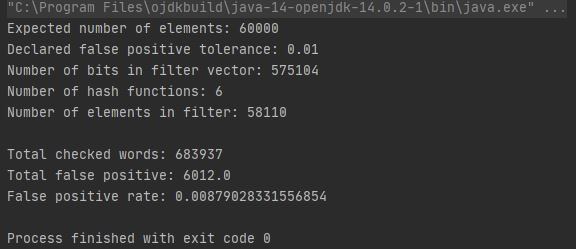
\includegraphics[width=\textwidth]{output}
\section*{Quellen}
\begin{itemize}
\item http://matthias.vallentin.net/blog/2011/06/a-garden-variety-of-bloom-filters/
\item https://github.com/google/guava/wiki/HashingExplained
\item https://iq.opengenus.org/applications-of-bloom-filter/
\item https://chromiumcodereview.appspot.com/10896048/
\end{itemize}
\end{document}




















